%\thispagestyle{plain}
\newgeometry{top=4cm, bottom=4cm, left=4cm, right=4cm} 

\setlength{\parindent}{2em}
\setlength{\parskip}{0em}
\setlength{\columnsep}{2em}
%\setcounter{page}{31}

\begin{multicols}{2}

%\small
\noindent
пересекает ось $Oz$ в различных точках. При $\phi = \pi$ образующая параллельна оси $Oz$.

Таким образом, пересекаться могут только такие пары образующих, которые лежат в одной вертикальной плоскости; иными словами, если одной из пересекающихся образующих соответствует угол $\phi$, то другой \linebreak 
соответствует угол $\phi + \pi$. Пусть \linebreak положение точки пересечения этих образующих определяется значе- \linebreak
ниями $\lambda_1, \lambda_2$ параметра $\lambda$. Тогда из (1) \\

\begin{cases}
x = (R + \lambda_1 \cos{\frac{\phi}{2}}) \cos{\phi} = \\
= - (R - \lambda_2 \sin{\frac{\phi}{2}}) \cos{\phi}, \\
y_1 = (R + \lambda_1 \cos{\frac{\phi}{2}}) \sin{\phi} = \\
= -(R - \lambda_2 \sin{\frac{\phi}{2}}) \sin{\phi}, \\
z = \lambda_1 \sin{\frac{\phi}{2}} = \lambda_2 \cos{\frac{\phi}{2}}.
\end{cases} \\

\noindent
Из этих выражений следует, что $\lambda_1, \linebreak
\lambda_2$ удовлетворяют системе уравнений \\

\begin{cases}
R + \lambda_1 \cos{\frac{\phi}{2}} = -R + \lambda_2 \sin{\frac{\phi}{2}}, \\
\lambda_1 \sin{\frac{\phi}{2}} = \lambda_2 \cos{\frac{\phi}{2}},
\end{cases} \\

\noindent
откуда при $\left(\phi \neq \frac{\pi}{2}, \frac{3\pi}{2}\right)$ находим $\displaystyle \lambda_1 = -2R \frac{\cos{\frac{\phi}{2}}}{\cos{\phi}}$. Подставив най- \linebreak
денное значение $\lambda_1$, в уравнения (1), получим координаты точки самопе- \linebreak
ресечения: \\

\noindent
$x = -R, y = -R \tg{\phi}, z = -R \tg{\phi}$. \\

\noindent
Отсюда видно, что при изменении $\phi$ точка самопересечения поверхности Мёбиуса движется вдоль прямой, которая лежит в плоскости $x = -R$ и описывается уравнением $z = y$. Таким образом, линия самопересече- \linebreak
ния является прямой (но не явля- \linebreak
ется образующей!). Отрезок этой \linebreak 
прямой изображен на обложке. Внимательно изучив заставку, вы найде- \linebreak
те линию самопересечения и на ней.

%\vfill\null
\columnbreak

\begin{Figure}
    \centering
    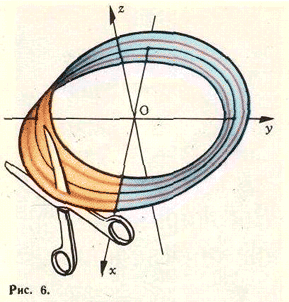
\includegraphics[width=\columnwidth]{pic1.png}
\end{Figure}

\noindent
\small
\textbf{Почему же лист Мёбиуса не \linebreak
распадается при разрезе?}

\noindent
%\normalsize
%Теперь нетрудно ответить и на этот вопрос. Рассмотрите на рисунке 4 (и на обложке) край ленты Мёбиуса, т.е. линию %$\lambda = \pm 1$. Присмотритесь: этот край не распадается на пару замкнутых кривых, как было бы в случае %неперекрученной полоски, а пред- \linebreak
%ставляет собой одну непрерывную кривую. Наш разрез не касался края, и поэтому край (а значит и вся полоска) после %разреза будет оставать- \linebreak
%ся целым куском. \\
Теперь нетрудно ответить и на этот вопрос. Рассмотрите на рисунке 4 (и на обложке) край ленты Мёбиуса, т.е. линию $\lambda = \pm 1$. Присмотритесь: этот край не распадается на пару замкнутых кривых, как было бы в случае неперекрученной полоски, а представляет собой одну непрерывную кривую. Наш разрез не касался края, и поэтому край (а значит и вся полоска) после разреза будет оставаться целым куском. \\

\noindent
%\small
\textbf{Как объяснить другие сюрпризы?}

\noindent
%\normalsize
Можно считать, что второй разрез осуществляется по линии $\lambda = \frac{1}{2}$ (рис. 6).

\noindent
Координаты точек на этой линии описываются (при $\phi \in [0, 2\pi]$) уравнениями \\

\begin{cases}
x = (R = \frac{1}{2} \cos{\frac{\phi}{2}}) \cos{\phi}, \\
y = (R + \frac{1}{2} \cos{\frac{\phi}{2}}) \sin{\phi}, \\
z = \frac{1}{2} \sin{\frac{\phi}{2}}.
\end{cases} \\

Очевидно, разрез делит нашу полоску на две части, которые можно условно назвать внешней и внутренней, причем внутренняя часть является такой же, только более узкой, полоской листа Мёбиуса. Что же представляет собой внешняя часть? \\

\centering
\footnotesize
\textit{Продолжение см. стр. 59}

\begin{flushright}
    \normalsize
    \textbf{31}
\end{flushright}



\end{multicols}